% Chapter Template


\chapter{Experiments} % Main chapter title

\label{experiments} % Change X to a consecutive number; for referencing this chapter elsewhere, use \ref{ChapterX}
We conducted several experiments on our human parts and keypoint detection module.
In fact, we applied the resulting network architecture from the human parts module later to the background extraction module.
All in all, we investigated eight network architecture variants differentiating in commonly discussed parameters.
For the keypoint detection module, we conducted tests with and without Dense layers.
On the human parts detection module, we tested the three state-of-the-art optimizers Adam, Nadam, and SGD and experimented with little
modifications to the SGD optimizer.
To overcome class invariance, we tried out three different loss functions of which one we have come up with
ourselves.
In the subsequent sections we will present our experimental setup, results, and constructive thoughts behind the studies.
%----------------------------------------------------------------------------------------
%	SECTION 1
%----------------------------------------------------------------------------------------

% with custom loss function and Adam optimizer_kps


%\section{Different Net Architectures}
\section{Ablation Study}



%-----------------------------------
%	SUBSECTION 1
%-----------------------------------

\begin{table}[]
\begin{footnotesize}
    \caption[Ablation Human Parts Module]{Ablation Human Parts Module: Network Architecture Comparison} \label{table:ablation}
\begin{tabular}{Nlllll}
\hline
\multicolumn{1}{|c}{} &
  \textbf{Name} &
  \textbf{\begin{tabular}[c]{@{}l@{}}Parameter \\ Amount\end{tabular}} &
  \textbf{\begin{tabular}[c]{@{}l@{}}Trainable \\ Parameters\end{tabular}} &
  \textbf{Layers} &
  \textbf{\begin{tabular}[c]{@{}l@{}}Training \\ Time/Epoch\end{tabular}} \\ \hline
\label{HRNet:traditional} & \begin{tabular}[c]{@{}l@{}}HRNet \\ \textit{- traditional}\end{tabular}          & 5,595,221 & 5,589,237 & 171 & 84.76s \\ \hline
\label{HRNet:filter} & \begin{tabular}[c]{@{}l@{}}HRNet \\ \textit{- adjusted filter}\end{tabular}      & 4,936,997 & 4,933,029 & 171 & 66.23s \\ \hline
\label{HRNet:3s} & \begin{tabular}[c]{@{}l@{}}HRNet \\ \textit{- 3 stages}\end{tabular}             & 848,409   & 846,441   & 100 & 82.33s \\ \hline
\label{HRNet:stride} & \begin{tabular}[c]{@{}l@{}}HRNet \\ \textit{- stride-down-up}\end{tabular}       & 4,953,269 & 4,949,157 & 177 & 63.21s \\ \hline
\label{HRNet:stride-i} & \begin{tabular}[c]{@{}l@{}}HRNet \\ \textit{- stride-down-up-input}\end{tabular} & 4,185,605 & 4,181,493 & 177 & 80.57s \\ \hline
\label{HRNet:add-i} & \begin{tabular}[c]{@{}l@{}}HRNet \\ \textit{- add-input}\end{tabular}            & 4,185,605 & 4,181,493 & 177 & 80.57s \\ \hline
\label{HRNet:add-dwconv} & \begin{tabular}[c]{@{}l@{}}HRNet \\ \textit{- add-depthwise-conv}\end{tabular} & 3,182,342 & 3,177,654 & 156 & 83.10s \\ \hline
\label{UNet} & UNet                                                                    & 656,389   & 654,261   & 88  & 85.37s \\ \hline
\label{HRNet:v3} & \begin{tabular}[c]{@{}l@{}}HRNet \\ \textit{- v3}\end{tabular}                   & 3,008,562 & 3,003,930 & 156 & 85.43s \\ \hline
\end{tabular}
    \end{footnotesize}
\end{table}
\setcounter{rowcntr}{0}


\subsection{Body Parts Detection Module }
\label{RBP}

In~\ref{fig:ablation-accuracy} we demonstrate our network architectures, which range from 88 until 177 layers and are
all fully convolutional networks.
For the HRNet \textit{(traditional)}~\ref{HRNet:traditional} we slightly deviate the HRNetV2 presented in~\cite{HRNetv2} by replacing the pooling
layers with strided-down and transposed convolutional layers.
The amount of levels and sizes of the feature maps correspond to~\ref{fig:custom_hrnet}.
As in HRNetV2 we use 4 stages with a filter size of 64 for each stage.
We add one level per stage starting with just the highest level $\mathcal{N}_L$
and concatenate the levels from stage 2 ongoing as demonstrated in HRNetV2.\\
For the HRNet \textit{(filters)}~\ref{HRNet:filter}, we adjust the filters in a way, so that higher levels use fewer filters then lower levels.
Additionally, we decrease the filters from the convolutional layers in the level blocks, starting from the highest filter
amount reducing until 36.
All levels are concatenated with a filter size of 36.\\
Subsequent architectures all make use of the adjusted filter amount.\\
For the HRNet \textit{(3 stages)}~\ref{HRNet:3s}, we only use the three first stages from~\ref{HRNet:filter} and omit
$\mathcal{N}_{XS}$.\
In HRNet \textit{(stide-down-up)}~\ref{HRNet:stride}, we stride down the Input from 240x320x3 to 120x160x36 and use this layer as Input layer
and highest Level $\mathcal{N}_L$. Lower layers scale relatively to $\mathcal{N}_L$.
The HRNet \textit{stride-down-up-input}~\ref{HRNet:stride-i} uses the initially strided down Input layer as input for
every stage instead of the concatenated results for lower levels.\\
As presented in the MobileNet paper~\cite{mobilenet} in~\ref{HRNet:add-dwconv} we experiment with depth-wise convolution
and replace the Concatenation layers after each stage with Add layers.\\
In the UNet~\ref{UNet} we use all levels and combine them via concatenation according to the traditional UNet~\cite{unet}.\\
Finally, we present our resulting high-to-low resolution network HRNet \textit{(v3)}~\ref{HRNet:v3}, where we fuse
the first stages and only concatenate the last stage. Furthermore, we conducted some adjustments to the layer amount
in the levels and stages as presented in~\autoref{method}.
\\\mbox{}\\
The HRNet stride-down-up~\ref{HRNet:stride} seems to train the fastest, when looking at~\ref{fig:ablation-correct-px} the
4.705kth step, it is only at three days and 13h closely followed by the traditional HRNet with the adjusted filters~\ref{HRNet:add-dwconv}
which is at 3 days and 13h. All other trainings took more than four days at that time.
However, one has to keep in mind that both trainings where conducted at the same dates, and the other dates differ.
So the server could have had other workloads, nevertheless, our trainings were the only ones running on the server most
of the time. This occasion as well is reflected in the training time of one epoch.
There as well both the HRNet \textit{stride-down-up} and HRNet \textit{adjusted-filter} only took about ~63, ~66 seconds,
where all the others took more then 80 seconds.
However, we would have expected the U-Net or HRNet \textit{3 stages} to be the fastest since they have the smallest
amount of layers and trainable parameters.
Further, the HRNet \textit{stride-down-up-input} contains less trainable parameters then \textit{stride-down-up}, so
we would have expected a faster training process here.
This verifies that the measurements are dependent from various circumstances.
Indeed, to improve comparability, we measured the third epoch to omit starting warm up phases.
\\\mbox{}\\
\paragraph{Comparison of network architectures}\mbox{}\\
%
The U-Net~\ref{UNet} has the smallest amount of layers with 88 and 654,261 trainable parameters.
The HRNet \textit{stride-down-up}~\ref{HRNet:stride} composes most trainable parameters with 4,949,157 and 177 layers, since the input
layer is first strided down and at the end transposed up again.
On the other hand, due to the reduced feature map sizes, this reduces the computation effort as well.
All comparison figures show very similar curves.
Since we could only run our experiments one complete training each, the results must be viewed circumspectly.
All figures~\ref{fig:ablation-accuracy, fig:ablation-correct-px, fig:correct-pixel-ratio} show very steep curves until
the 500th episode and start to flatten then.\\
When looking at~\ref{fig:train-img-0} and~\ref{fig:train-img-20} this steep initial increase is visually reflected.
When after the first episode the circumferences of the body shapes are predicted vaguely, after the 20th episode the
networks have already learned to predict the locations of body parts relatively close.
Of course, there has to be regarded, that the different predictions were made on different poses, which might differ in
their complexity.
Nevertheless, the UNet~\ref{UNet} and the HRNetV3~\ref{fig:hp_accuracy_hrnet_v3} seem to accomplish superior performance.
After the first episode, the body shape is already estimated precisely close to the input image.
HRNetV3 even shows correct class estimations for different body parts such as the torso, head, arms, and legs already.
In the 20th episode then the labels seem to be estimated very close to the true labels.

\begin{figure}[H]
    \centering
    \includegraphics[width=\textwidth, height=\textheight, keepaspectratio]{Figures/ablation_study_hp_accuracy.png}
    \decoRule
    \caption[Ablation Human Parts Module: Accuracy]{Ablation Human Parts Module: Accuracy Comparison}
    \label{fig:ablation-accuracy}
\end{figure}

The accuracy graph shows that the HRNet \textit{traditional} and HRNetV3 get the best results from epoch 500 onwards.
At step 55.55k they reach 99 percent.
However, the HRNet \textit{stride-down-up} has a lower curve until the 4.3kth epoch, it then makes a jump in Accuracy
and at the end reaches 99 percent as well.
Interestingly the U-Net with the by far fewest parameters and layers does receive very good results as well making almost
99 percent in Accuracy at the end.
The HRNet with only three stages shows the lowest curve and reaches only 98.87 percent points on accuracy at the end.

\begin{figure}[H]
    \centering
    \includegraphics[width=\textwidth, height=\textheight, keepaspectratio]{Figures/ablation_study_hp_correct_pixel.png}
    \decoRule
    \caption[Ablation Human Parts Module: Correct Pixel]{Ablation Human Parts Module: Correct Pixel}
    \label{fig:ablation-correct-px}
\end{figure}

The correct pixel graph~\ref{fig:ablation-correct-px} measures how many pixels of the 240x320 image where predicted correctly
in one batch. The maximum which could be reached here is $240\times320\times3=\numprint{230400}$.
Since the single epochs vary a lot, it makes more sense to look at the smoothed results.
The curves again are very close to each other, with the best results coming from the HRNetV3 with $\numprint{219670}$ and
the HRNet \textit{traditional} with $\numprint{219640}$.
The lowest curve again shows the HRNet \textit{3 stages}.

\begin{figure}[H]
    \centering
    \includegraphics[width=\textwidth, height=\textheight, keepaspectratio]{Figures/ablation_study_hp_bp_pixel_ratio.png}
    \decoRule
    \caption[Ablation Human Parts Module: Correctness Ratio]{Ablation Human Parts Module: Correct Pixel Ratio}
    \label{fig:correct-pixel-ratio}
\end{figure}

For~\ref{fig:correct-pixel-ratio} we summed up the amount of body part pixels and divided by the amount of correctly
predicted pixels for one training batch.
This figure as well displays high variances for the different epochs, which is why it is important to take the smoothed
values into account. We receive similar courses as already inspected in~\ref{fig:ablation-correct-px}.
The HRNet \textit{traditional} and HRNetV3 take the lead wih the \textit{traditional} being slightly above the HRNetV3
with 0.05 percent points. With 31.44 percent the HRNet \textit{traditional} shows the best results, whereas HRNet
\textit{3 blocks} performs worst with 30.38 percent at step 4.93k.

\begin{figure}[H]
    \centering
    \includegraphics[width=\textwidth, height=\textheight, keepaspectratio]{Figures/ablation_study_train_imgs_0.png}
    \decoRule
    \caption[Ablation Human Parts Module: 1st Episode Predictions]{Predicted images of network architectures after first
    episode}
    \label{fig:train-img-0}
\end{figure}
\begin{figure}[H]
    \centering
    \includegraphics[width=\textwidth, height=\textheight, keepaspectratio]{Figures/ablation_study_train_imgs_20.png}
    \decoRule
    \caption[Ablation Human Parts Module: 20th Episode Predictions]{Predicted images of network architectures after 20th
    episode}
    \label{fig:train-img-20}
\end{figure}

\paragraph{Summary}\mbox{}\\
In summary, our experiments show that our constructed HRNetV3 performs best, and the HRNet with only three stages performs
worst.
Interesting here would be different variations in the level of feature map sizes.
For instance what would happen if the level $\mathcal{N}_{XS}$ was maintained as smallest level and the level
$\mathcal{N}_M$ was strided down slightly more?
Insightful as well is the performance of the UNet, which has less than half of trainable parameters and layers compared to
the HRNet \textit{traditional} or HRNetV3, but does not perform much worse.\\
Additionally, further tweaks and studies in these network architectures applied to our different modules would be
greatly enlightening.


%-----------------------------------
%	SUBSECTION 2
%-----------------------------------
\subsection{Joint Detection Module }

\begin{table}[H]

%\begin{footnotesize}
    \caption[Ablation Keypoint Module]{Ablation Keypoint Detection Module: Network Architecture Comparison} \label{table:ablation-kp}
\begin{tabular}{|Nlllll|}
    \hline
\multicolumn{1}{|c}{} &
  \textbf{Name} &
  \textbf{\begin{tabular}[c]{@{}l@{}}Parameter \\ Amount\end{tabular}} &
  \textbf{\begin{tabular}[c]{@{}l@{}}Trainable \\ Parameters\end{tabular}} &
  \textbf{Layers} &
  \textbf{\begin{tabular}[c]{@{}l@{}}Training \\ Time/Epoch\end{tabular}} \\ \hline
\label{kps-dense-blockl} & \begin{tabular}[c]{@{}l@{}}KPS-Dense \\ \textit{- block\_L}\end{tabular}          & 221,748,579 & 218,735,769 & 51 & 68.75s \\ \hline
\label{kps-dense} & \begin{tabular}[c]{@{}l@{}}KPS-Dense\end{tabular}      & 23,097,980 & 20,086,328 & 13 & 67.05s \\ \hline
\label{kps-hrnet} & \begin{tabular}[c]{@{}l@{}}KPS-FCN\end{tabular}             & 4,119,529 & 1,109,991 & 41 & 63.78s \\ \hline
\end{tabular}
    %\end{footnotesize}
\end{table}
\setcounter{rowcntr}{0}

\paragraph{Network Architectures}\mbox{}\\
We created three variations of keypoint detection network architectures of which two\ref{kps-dense, kps-dense-blockl}
utilize Dense layers to estimate the keypoint locations and KPS-FCN~\ref{kps-hrnet} implements the third stage of our
build HRNetV3.\\
KPS-Dense~\ref{kps-dense-blockl}, additionally to the dense stage, utilizes the third stage of the HRNetV3.\\
The dense stage first uses max pooling to reduce the feature map size from 240x230x9 to 120x160x1, 58x78x32, and then 28x38x64.
The resulting pooling layer is flattened and followed by two dense layers, which are combined with AlphaDropout and
batch normalization.
The layers include 1024 and 512 units.
The first Dense layer is connected to a Softmax activation function,
the second to a linear activation function. The model estimates 38 x,y coordinates for the keypoint locations.
The networks loss function calculates the distance from the predicted keypoint locations to the true locations and optimizes
the networks via mean-squared-error.\\
In fact, the KPS-FCN~\ref{kps-hrnet} only uses convolutional layers.
The true labels calculate gaussians with a radius size of three for the locations of the keypoints.
We combined the keypoint classes for equal body locations such has legs and arms, resulting in 11 joint classes.
This network predicts 11 different labels for the classes. The network is optimized as well with mean-squared-error.

All networks are trained with an Adam optimizer and a learning rate of 0.001 and run for 5556 epochs.

\begin{figure}[H]
    \centering
    \includegraphics[width=\textwidth, height=\textheight, keepaspectratio]{Figures/ablation_study_kps_imgs.png}
    \decoRule
    \caption[Ablation Keypoints Detection Module: Predicted Training Images]{Predicted images of keypoint detection networks
    after first, 20th and last episode}
    \label{fig:kps-train-imgs}
\end{figure}

Both figures~\ref{fig:kps-map-loss},~\ref{fig:kps-loss} show similar curves.
Until the 500th episode they decrease steeply and then they start to flatten.
KPS-Dense~\ref{kps-dense} has the fewest layers with 13, however KPS-FCN~\ref{kps-hrnet} contains only 1,109,991
trainable parameters, the dense networks train \~20/ \~218 times more parameters.
The networks only differ slightly in their training epoch time and are all between 63 and 69 seconds.\\
The main difference though is visible in the predicted training images in~\ref{fig:kps-train-imgs}.
The keypoint detection modules seem not to learn the locations of the body parts, but that the probability of the location
of a keypoint being at the center of the image is much more likely than outer locations.
Very interesting about the KPS-FCN is that this network first learns the locations of the feet, and then slowly goes
upward per epoch learning the other keypoint locations in a continuous way.


\begin{figure}[H]
    \centering
    \includegraphics[width=\textwidth, height=\textheight, keepaspectratio]{Figures/ablation_study_kps_map_loss.png}
    \decoRule
    \caption[Ablation Keypoints Detection Module: Loss FCN]{Ablation Keypoints Detection Module: Loss FCN}
    \label{fig:kps-map-loss}
\end{figure}


\begin{figure}[H]
    \centering
    \includegraphics[width=\textwidth, height=\textheight, keepaspectratio]{Figures/ablation_study_kps_loss.png}
    \decoRule
    \caption[Ablation Keypoints Detection Module: Loss Dense Layers]{Ablation Keypoints Detection Module: Loss Dense Layers}
    \label{fig:kps-loss}
\end{figure}

%-----------------------------------
%	SECTION 2
%-----------------------------------




\subsection*{Experiments with optimizers}
We conducted our training with Mini-Batch Gradient Descent with a batch size of three.
In addition, we will present some mathematical backgrounds of optimizer algorithms and explain further aspects of
SGD in more detail.
\begin{figure}[H]
    \centering
    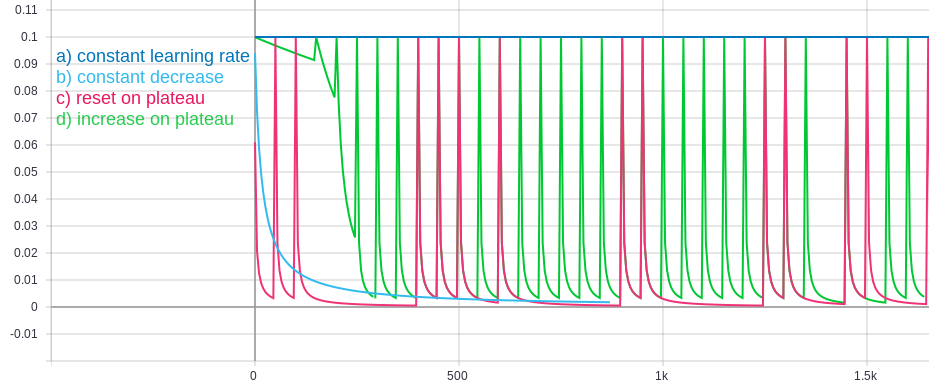
\includegraphics[width=\textwidth,height=\textheight,keepaspectratio]{img/learning_rate2.png}
    \decoRule
    \caption[Experiments: Learning Rate SGD]{Experiments with Learning Rate SGD.}
    \label{fig:sgd-learning-rate}
\end{figure}
In our experiments we tested SGD, Adam, and Nadam all with initial learning rates of $\eta=0.001$.
We configured SGD to use Nesterov Momentum with a value of $\gamma=0.9$, Adam with epsilon $\epsilon=1e-7$ and AMSGrad.
Nadam used the exponential decay parameters $\beta_1=0.9; \beta_2=0.999$ and epsilon $\epsilon=1e-7$.
Additionally, we conducted several tests with the learning rate in SGD and its influence on the training process.
One SGD configuration is with a constant learning rate $\eta$, one decays with $\eta=0.01$, and one learning rate
decays with $\eta=0.01$, but will reset to the initial learning rate, when no significant learning or changes regarding
the loss value is observed over the last 50 epochs anymore.
Another experiment with SGD increases the ascent of decay when a plateau is hit with increasing decay values
$[1e-5, 1e-4, 1e-3, 1e-2]$ as visualized in ~\ref{fig:sgd-learning-rate}.



% https://ruder.io/optimizing-gradient-descent/index.html#nadam

%The goal of gradient descent is to find the minima of the weights, so that the overall error is minimized.
%
%The learning rate is one of the important hyper-parameters, which determines how quickly this minimum can be reached.
%It sets the step size and with it the amount of steps until the model converges.
%So it additionally decides about the training length of the network~\cite{deeplcomputervision}.




%https://mlfromscratch.com/optimizers-explained/#/

\subsubsection*{Comparison of Adam, Nadam and SGD}
\begin{figure}[H]
    \centering
    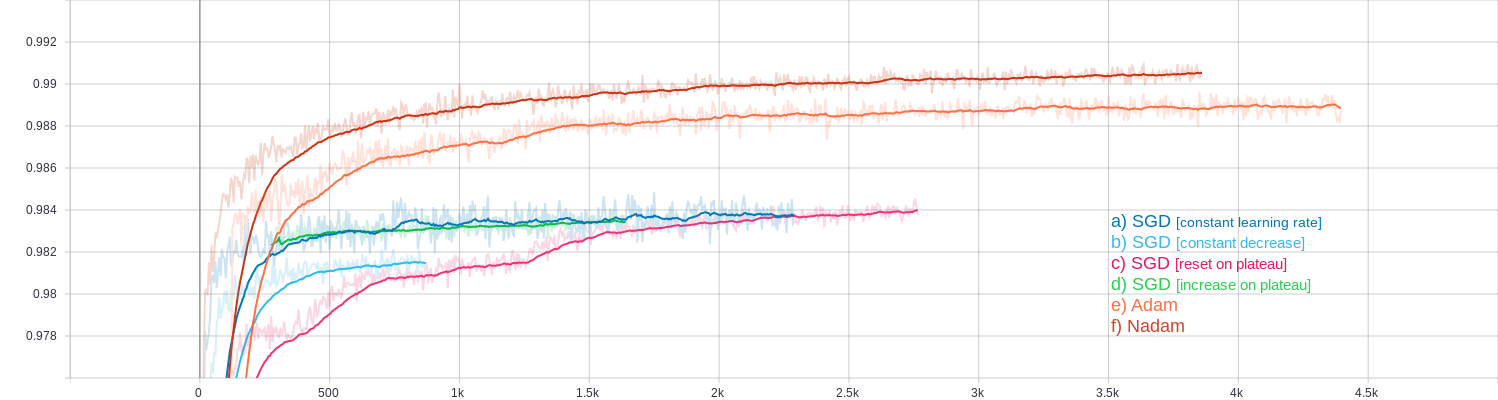
\includegraphics[width=\textwidth,height=\textheight,keepaspectratio]{img/accuracy_all.png}
    \decoRule
    \caption[Experiments: Accuracy]{Accuracy of different optimizer settings}
    \label{fig:accuracy}
\end{figure}

The Figure on accuracy~\ref{fig:accuracy} shows that our network makes huge learn progress in the first
200 to 300 epochs with an ascent of almost 90 degrees.
However, the graph shows that SGD performs worse than Adam or Nadam, all networks reach a commendable accuracy above
98 percent, whereas Nadam even gets over the 99 percent mark.
Adam and Nadam start to flatten a little bit later than SGD about 100 epochs.
Furthermore, their curves flatten more evenly, whereas SGD
seems to flatten more abruptly.
Interestingly, the SGD optimizer, where we reset the learning rate on plateau, shows jumps in its curve.
There one can observe the typical flattening of SGD and then, when a reset took place, the learning process starts again.
This indicates that SGD hit local minima from which it seems to jump out and re-trigger the adjustment of $\theta$.

%\begin{figure}[H]
%    \centering
%    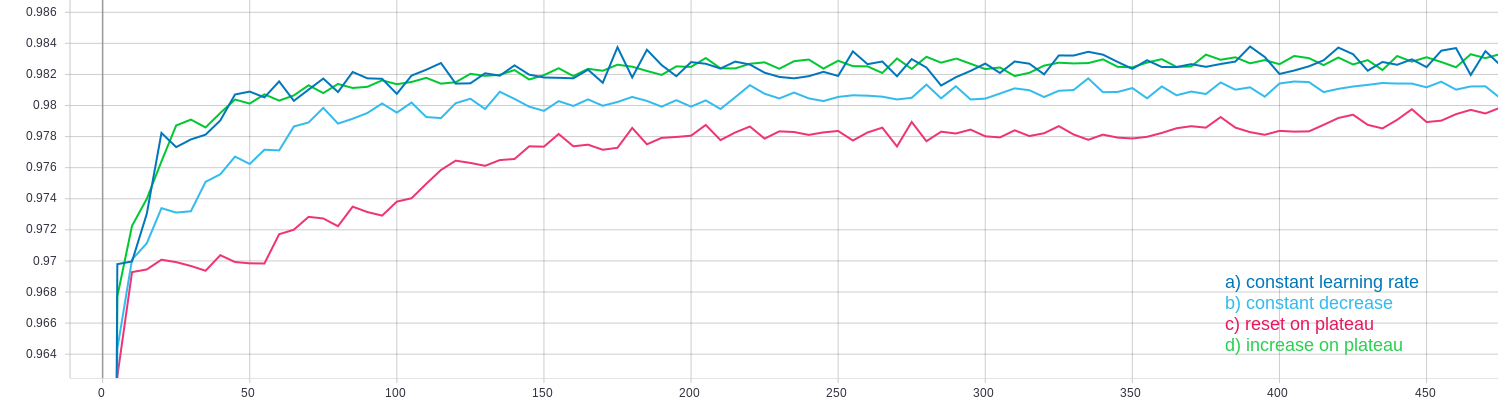
\includegraphics[width=\textwidth,height=\textheight,keepaspectratio]{img/accuracy_sgd.png}
%    \decoRule
%    \caption[Accuracy SGD]{Accuracy SGD.}
%    \label{fig:sgd-accuracy}
%\end{figure}



%\begin{figure}[H]
%    \centering
%    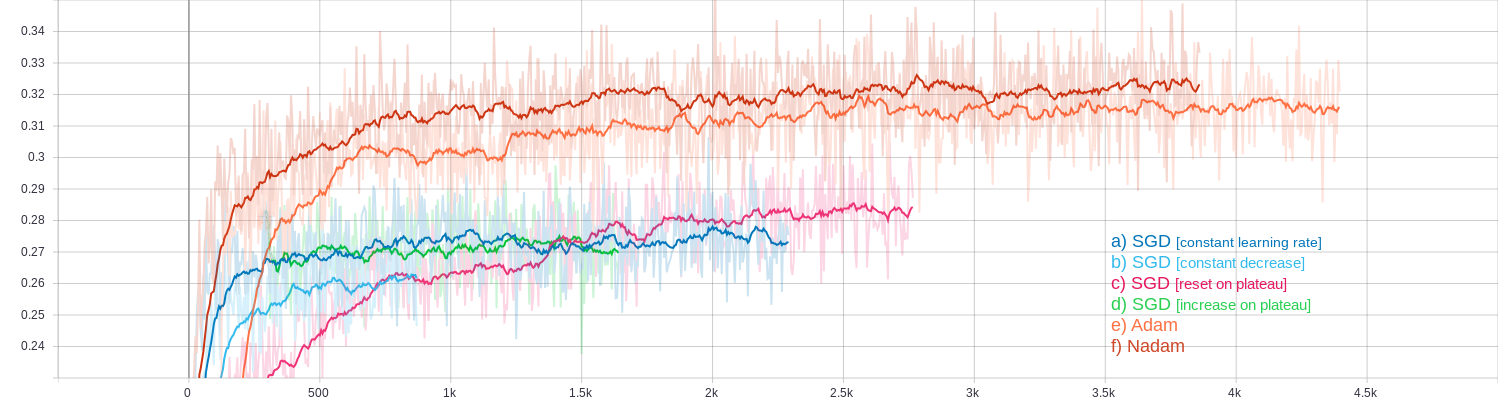
\includegraphics[width=\textwidth,height=\textheight,keepaspectratio]{img/accuracy_body_part_all.png}
%    \decoRule
%    \caption[Correct BPR]{Correct body part pixel relation}
%    \label{fig:acc-bp}
%\end{figure}


\begin{figure}[H]
    \centering
    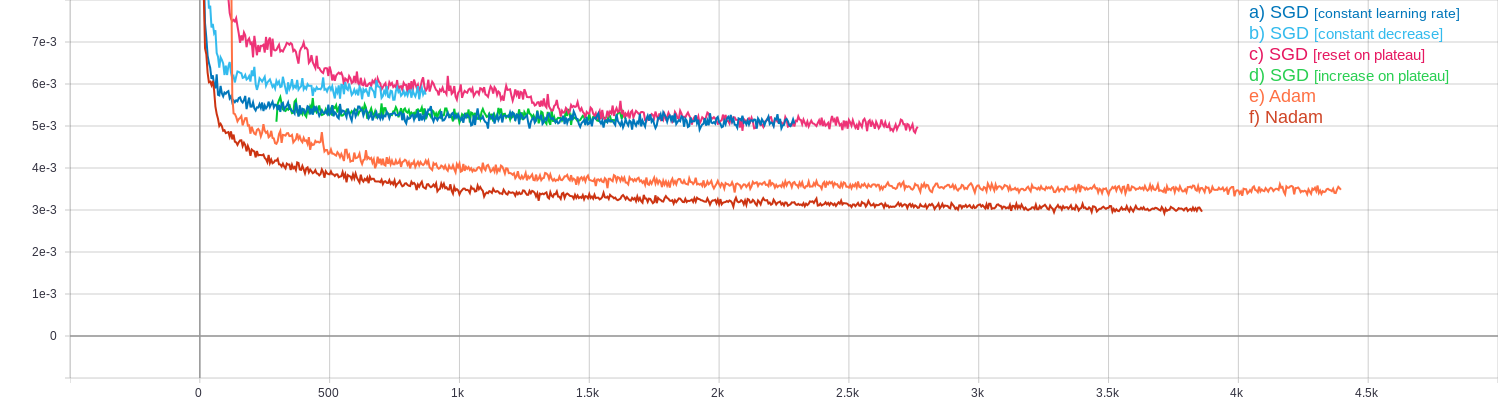
\includegraphics[width=\textwidth,height=\textheight,keepaspectratio]{img/loss_all.png}
    \decoRule
    \caption[Experiments: Loss curves]{Experiments: Loss curves}
    \label{fig:loss}
\end{figure}
Similar process curve trends can be observed in~\ref{fig:loss}, while the curves are mirrored at the x-axis.
This correlation of loss and accuracy trend proves the associate learning process for the different optimizers.
\\\mbox{}\\
\paragraph{Conclusions}\mbox{}\\
Our results are reflected by the research from Choi et Al~\cite{empiricaloptimizers}.
They conducted very interesting research with the thesis that more general optimizers would never underperform
the ones they approximate.
Meaning RMSProp, Adam and Nadam would always perform at least as good if not better than Momentum, Nesterov or SGD.
They impose to carefully tune the hyperparameters and not just conclude an optimizer would work better than another one.
This is why we used very commonly recommended hyperparameters.
A continuing grid search could help to find an even more efficient way for training and probably even result in better
learned network parameters $\theta$.
%\begin{figure}[H]
%    \centering
%    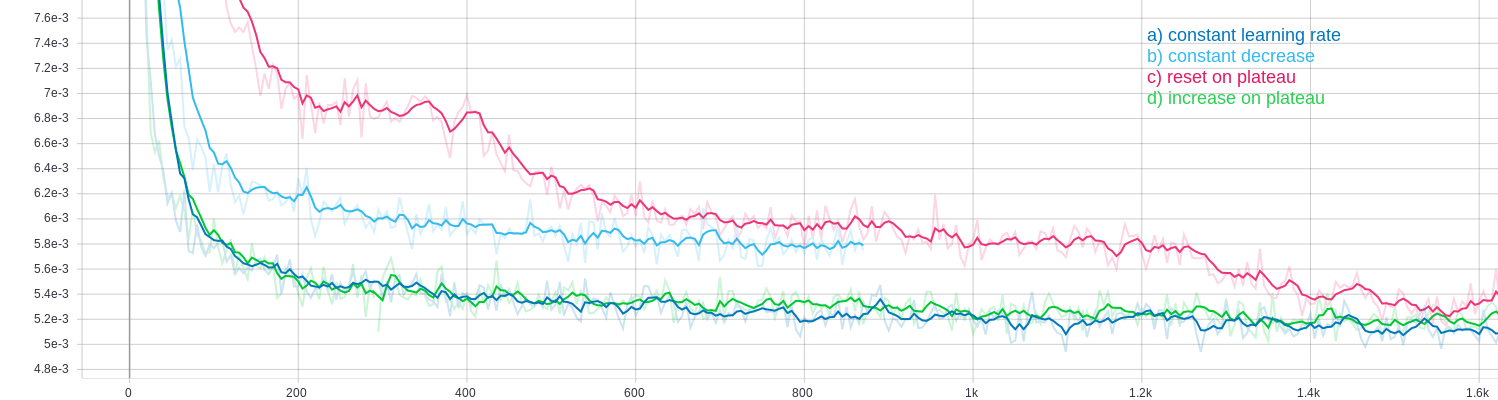
\includegraphics[width=\textwidth,height=\textheight,keepaspectratio]{img/loss_sgd.png}
%    \decoRule
%    \caption[Loss SGD]{Loss SGD.}
%    \label{fig:sgd-loss}
%\end{figure}



%----------------------------------------------------------------------------------------
%	SECTION 3
%----------------------------------------------------------------------------------------


\section{Performance of loss functions}

As already mentioned in~\autoref{optimizers} loss functions $\mathfrak{J}$ closely work together with optimizer algorithms.
The loss function is used in the optimizer algorithm as seminal feedback deciding about the success of the learning process of a
neural network.
It calculates how close a prediction $y_p$ from a neural network is to the true label $y_t$.

\subsection{Commonly used loss functions}
One classical loss function is Mean Squared Error (MSE).
The error represents the difference between $y_t$ and $y_p$.
MSE then squares the error to even out negative results and calculates the sum of all these errors.
For our fully convolutional network, each pixel presents a certain class.
As visualized in~\ref{fig:feature-maps-output}, our Human Parts module predicts nine classes.
This means, there are nine labels possible for each pixel.
Now, the neural network estimates with a certain probability of how likely a certain class would be true for a specific pixel.
The error then calculates the difference between the estimation or prediction and the true label, which includes a
value of 1 only for the true class.
Additionally to the summation of squared errors, MSE divides this sum with the number of all squares resulting in the mean
value:

\begin{align}
    MSE(y_t,y_p) = \frac{1}{n}\cdot\sum_[i=1]^n(y_t-y_p)^2
\end{align}

We trained the Keypoint Detection and Body Part Extraction modules with MSE.

However, with our Body Part Detection Module we initially had problems with class imbalances.
First, we conducted our training with Sparse Categorical Cross Entropy (SCCE), which is a common loss function used in image
segmentation.
Wrong predictions are weighed harder, especially the ones with a great wrong probability value.
This is accomplished by calculating the logarithm of the predicted values.
Since the logarithm function $log(x)$ is negative for $x \in \Re and [0>x>1]$, and input values closer to zero mean
an exponential decrease towards $-\infty$ and there is just one true label for the different classes of one pixel, if
the prediction is clearly the wrong class, the cost will be exponentially higher.

\begin{align}
    SCCE(y_t,y_p) = -\sum_{i,j=1}^{i,j}y_{t_{i,j}}\cdot log(y_{p_{i,j}})
\end{align}
Here \textit{i,j} stands for the column and row pixels of the image.

Nevertheless, our first results~\ref{fig:cross_entropy_pred_img} made us believe that with SCCE our net was not able to
learn the correct labels for the pixels.
Especially the prediction after the 60th epoch shows, that the net mainly has learned to classify all body parts with the
torso class.
We assumed this was the case, because the likeliness of the pixel to be of class torso is higher than, for
example, foot.
Furthermore, however, the accuracy graph shows descent results over 94 percent it started to flatten more and more becoming
almost flat after the 50th epoch already.
\begin{figure}[H]
    \centering
    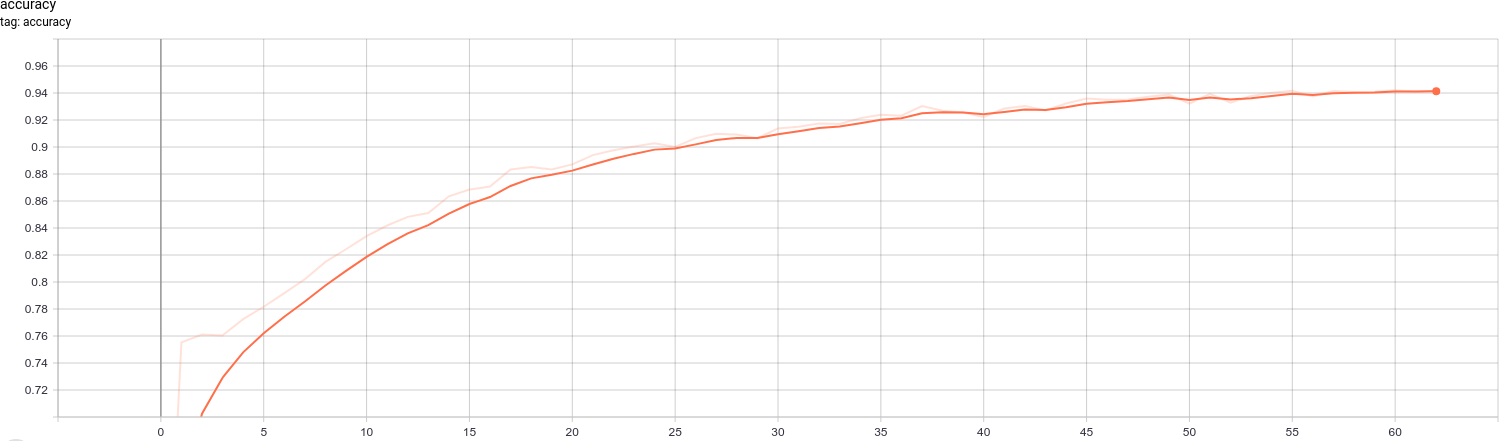
\includegraphics[width=\textwidth,height=\textheight,keepaspectratio]{Figures/accuracy_cross_entropy.png}
    \decoRule
    \caption[Loss Functions SCCE: Accuracy]{Accuracy for training with Sparse Categorical Cross Enntropy loss function}
    \label{fig:accuracy_cross_entropy}
\end{figure}
\begin{figure}[H]
    \centering
    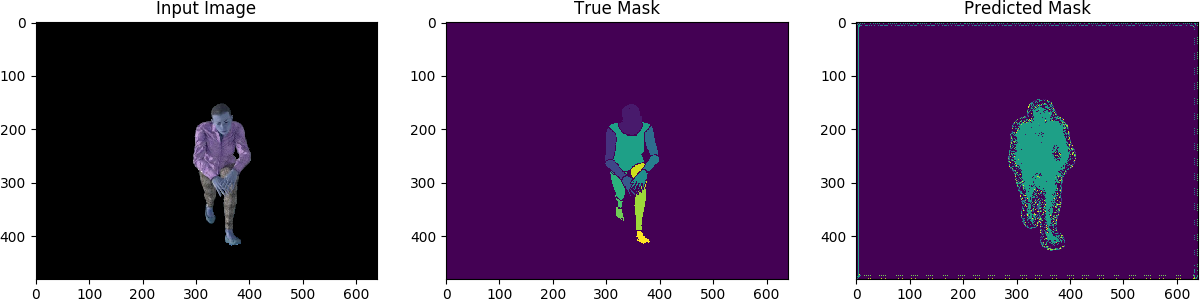
\includegraphics[width=\textwidth,height=\textheight,keepaspectratio]{Figures/crossentropy_imgs_prediction_last_epoch.png}
    \decoRule
    \caption[Loss Functions SCCE: predictions]{Predicted images for training with Sparse Categorical Cross Entropy loss function}
    \label{fig:cross_entropy_pred_img}
\end{figure}
We then created our own loss function for this class imbalance problem as explained in~\autoref{ciloss}.
Moreover, we reduced the number of classes from 14 to nine accumulating left and right body parts such as foot and arm.
A later experiment shows, on the contrary, that our build network HRNetv3 even learns slightly better than with our own created
loss function CILoss~\ref{fig:ablation-accuracy}.
Even though, this of course could be by chance due to current training circumstances.


\subsection{Our custom loss function CILoss}
\label{ciloss}
This loss function confronts the problem of class imbalance, which especially occurs in body part recognition.
The background pixels appear most often, and the different body part classes occur much less often and they even
differ a lot in their relative occurrence.
\\\mbox{}\\
We try to confront this problem with a weighed map $\mu$, which takes the body parts as a graph and calculates
the distances from each body part $b_x$ to all other body parts $b_n$, and store this data inside a table.
This weighed map $\mu$ is applied to the true labels of $y_{true}$ so that wrong predictions further away from the true
class will be punished more. For example if the network predicts hand instead of lower arm, the error will be less as if
the network predicts foot.
\\\mbox{}\\
Additionally, this weight map is evened out with a multiplier to reduce the distances and facilitate
the learning process for the network.
\\\mbox{}\\
As in MSE we calculate the difference $\mathcal{E}$ between $y_t$ and $y_p$, but do not square the result, we just use the absolute value.
We multiply the resulting error $\mathcal{E}$ with our weighed map receiving $\delta$.
To calculate the loss we then sum the error $\mathcal{E}$ and delta $\delta$ pixel-wise:

$$\mathcal{E}=y_t(x)-y_p(x)$$
$$\delta=\theta\cdot\mu[argmax(y_t)] $$
$$L=\sum_{i=0}^{n}\mathcal{E}_i+\delta_i$$


\begin{figure}[H]
    \centering
    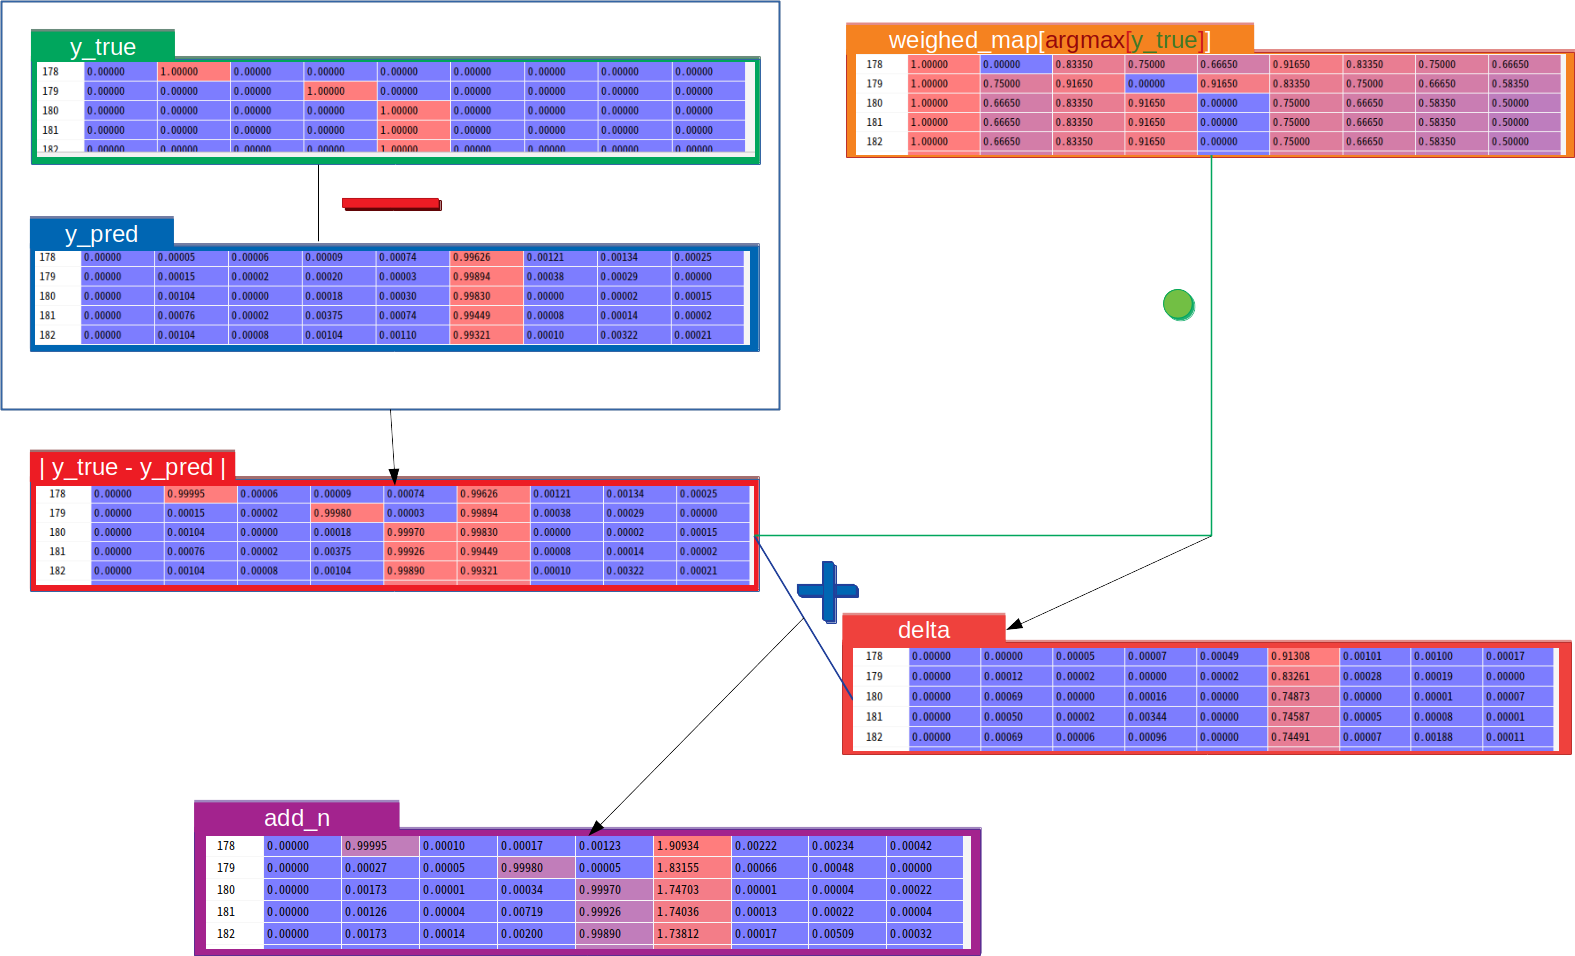
\includegraphics[width=\textwidth,height=\textheight,keepaspectratio]{img/loss_calculation.png}
    \decoRule
    \caption[Loss Functions CILoss: Calculation]{Visualization of our custom loss function CILoss}
    \label{fig:ciloss-calc}
\end{figure}
